\chapter{Implementación del Sistema de Protección por Corriente}
\lineaLateral

\begin{resumenCapitulo}
Este capítulo detalla el diseño y la implementación del sistema de protección activa del brazo robótico mediante el uso del sensor de corriente ACS712, integrads estratégicamente para supervisar el consumo eléctrico y prevenir fallas térmicas o mecánicas. 

Se describe la arquitectura del sistema desde su conexión electrónica hasta su procesamiento lógico, destacando el desarrollo de una interfaz en LabVIEW para el monitoreo en tiempo real. Este enfoque permite que el sistema actúe como un disyuntor inteligente, capaz de detectar sobreesfuerzos y ejecutar protocolos de seguridad automáticos, garantizando así la integridad de los motores y la eficiencia operativa de la estructura.
\end{resumenCapitulo}

\section{Lista de materiales}
\begin{itemize}
	\item Sensor ACCS712.
	\item Motores del brazo robótico.
	\item Multímetro.
	\item Drivers BTS7960.
	\item Labview Community 2025.
	\item Arduino Uno.
\end{itemize}


\section{Picos de Corriente en Actuadores DC}

El comportamiento eléctrico de los motores de corriente continua presenta variaciones críticas durante las etapas transitorias de operación. Al iniciar el movimiento, se produce un fenómeno conocido como \textit{Inrush Current} o corriente de irrupción, donde el motor demanda una intensidad significativamente superior a su valor nominal debido a la ausencia de fuerza electromotriz inversa (f.e.m.) y a la inercia mecánica inicial. 

De igual manera, los frenados bruscos y las inversiones de giro generan picos de corriente. La monitorización de estos transitorios es vital, ya que picos no controlados pueden degradar prematuramente las pistas de potencia y los componentes del sistema.



\section{Seguridad Operativa: Detección de Colisiones y Obstrucciones Mecánicas}

Más allá del monitoreo preventivo, el sensor ACS712 se integra como un fusible inteligente dentro de la arquitectura de control. En una colisión o bloqueo mecánico, el motor entra en una condición de rotor bloqueado (\textit{stall current}), elevando la corriente de forma exponencial al intentar vencer la resistencia física. 

Al procesar esta señal en el Arduino Uno, es posible programar una respuesta inmediata que desconecte la alimentación mediante el relevador antes de que ocurra un daño irreversible. A diferencia de un fusible térmico convencional, este sistema permite ajustar los umbrales de detección mediante software (setpoints), gracias a ello, se puede distinguir entre un pico de arranque normal y una obstrucción crítica por colisión.

\section{Detección de Anomalías Eléctricas: El Sensor ACS712}
% Habla aquí de por qué el ACS712 es mejor que un fusible térmico (es rearmable y más rápido).
% Explica el intento con el pin de sensado del BTS7960 y por qué el ACS712 dio mejor lectura.

La seguridad del sistema robotizado depende de una respuesta inmediata ante fallas eléctricas. Tomando como base el análisis del capítulo anterior, donde se calculó que en el escenario de carga máxima y usando su voltaje nominal de 24 V, los motores pueden demandar hasta \textbf{14 A}, se implementó el sensor de efecto Hall \textbf{ACS712}. Este dispositivo ofrece una protección mediante software y un monitoreo en tiempo real del consumo energético. 

A diferencia de la respuesta lenta y destructiva de un fusible, el ACS712 permite identificar si una articulación está experimentando un sobreesfuerzo o si el ciclo de trabajo se mantiene dentro de los parámetros de eficiencia diseñados. Una vez detectada y corregida cualquier anomalía, el sistema puede retomar su actividad de forma automática, eliminando la necesidad de reemplazar componentes físicos y garantizando una mayor disponibilidad del robot.

\subsection{Comparativa de Sensado: BTS7960 vs. ACS712}

Para la gestión de potencia de los motores DC del brazo robótico, se seleccionaron los módulos BTS7960. Originalmente, se pretendía aprovechar la función de diagnóstico de corriente integrada en el BTS7960. Se desarrolló un algoritmo para el Arduino Uno para procesar las señales analógicas emitidas por el pin de sensado del módulo; sin embargo, las lecturas obtenidas carecían de consistencia y precisión. Este fenómeno se atribuye a que el sensor del BTS7960 está optimizado para cargas elevadas, con un umbral operativo ideal a partir de los \textbf{5 A}. Como se detalla en la \textbf{Figura \ref{fig:tabla_motores}}, los motores del Move Master EX operando a 24V demandan un máximo de \textbf{2.75 A}. 

\begin{itemize}
	\item \textit{Nota técnica:} Debido a que en este diseño se ha optado por alimentar el sistema a \textbf{12 V}, el consumo de corriente es proporcionalmente menor al nominal, alejando aún más la señal del rango de precisión del sensor integrado en el driver.
\end{itemize}

\begin{figure}[h]
	\centering
	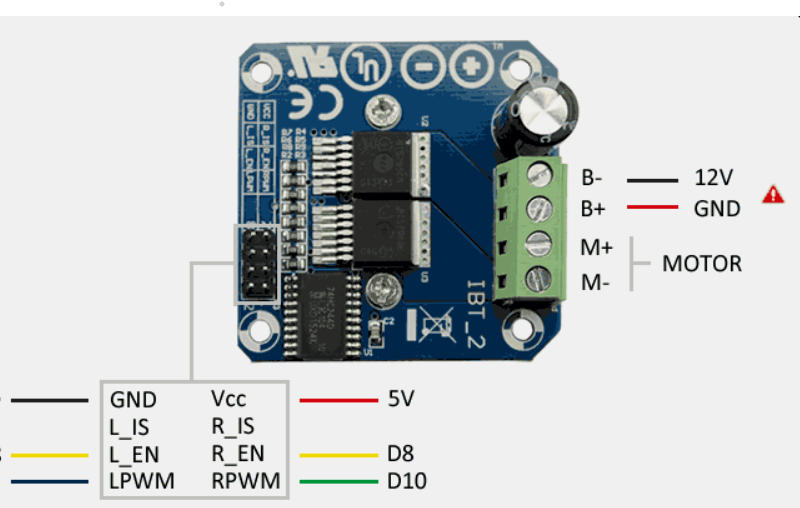
\includegraphics[height=0.28\textheight, keepaspectratio]{images/SensorCorriente/screenshot011}
	\caption[Pines del driver BTS7960]{Pines del driver BTS7960. \cite{LuisLlamas}}
	\label{fig:sPinesBts7960}
\end{figure}

\begin{figure}[h]
		\centering
	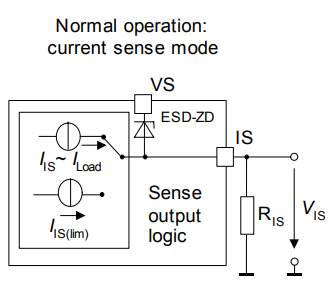
\includegraphics[height=0.3\textheight, keepaspectratio]{images/SensorCorriente/screenshot012}
	\caption[Medición de corriente en el driver BTS7960]{Medición de corriente en el módulo BTS7960. A la salida se obtiene un voltaje proporcional a la corriente suministrada por el chip. \cite{BTS7960Datasheet} }
	\label{fig:screenshot012}
\end{figure}



\begin{figure}[h]
		\centering
	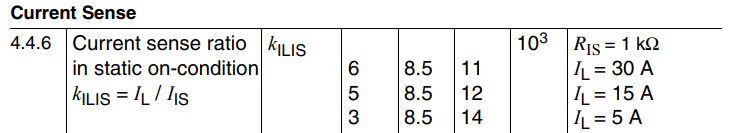
\includegraphics[width=1\linewidth]{images/SensorCorriente/screenshot013}
	\caption[Especificaciones de corriente del pin del módulo BTS7960]{Especificaciones de corriente del pin del módulo BTS7960. La mínima corriente es de 5 Amp, por lo que no se garantizan medidas precisas debajo de ese valor. \cite{BTS7960Datasheet} }
	\label{fig:screenshot013}
\end{figure}


Ante esta limitante, se decidió integrar el sensor de corriente externo \textbf{ACS712ELCTR-20A-T}. Este dispositivo basado en el efecto Hall permite medir rangos de corriente entre \textbf{-20 A y 20 A} con una sensibilidad de \textbf{100 mV/A}. Se eligió por poseer una resolución adecuada para la demanda real de los motores, el ACS712 garantiza una medición lineal y confiable para la protección del sistema.

\begin{figure}[h]
	\centering
	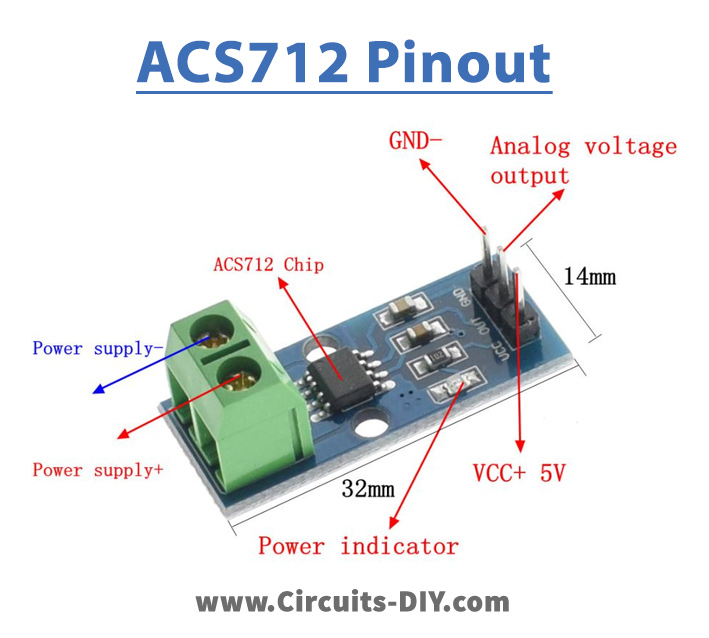
\includegraphics[width=0.7\linewidth]{images/SensorCorriente/screenshot014}
	\caption[Pines del ACS712]{Pines del ACS712. Es un sensor que brinda una señal analógica dependiendo de la corriente suministrada a su entrada.}
	\label{fig:screenshot014}
\end{figure}

\begin{figure}[h]
	\centering
	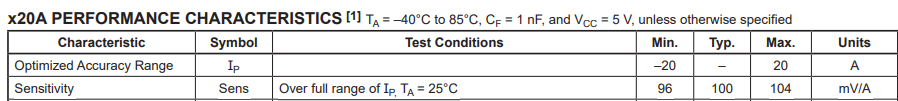
\includegraphics[width=1\linewidth]{images/SensorCorriente/screenshot015}
	\caption[Hoja técnica del sensor ACS712]{Datos técnicos sobre el sensor. Su sensibiliad técnica es de 100mV/A con un rango de lectura de -20 a 20 Amp. \cite{ACS712Datasheet}}
	\label{fig:screenshot015}
\end{figure}


\section{Integración del ACS712}
Debido a que los sensores de diagnóstico integrados en los controladores BTS7960 no proporcionaron lecturas consistentes para el rango de operación del robot, se descartó su uso en favor de una solución más robusta y centralizada. En su lugar, se optó por integrar un único sensor de corriente ACS712 ubicado estratégicamente en la línea principal de alimentación de corriente directa. Este sensor se encarga de monitorear el flujo de energía proveniente de la fuente de poder de 12 Vcc, permitiendo supervisar el consumo total del sistema y actuar como una barrera de seguridad global ante cualquier sobreesfuerzo o anomalía eléctrica en los actuadores.


\subsection{Cálculos}
Según la hoja de datos del sensor \cite{ACS712Datasheet}, tiene un offset de voltaje $V_{OE}$ que equivale al voltaje de alimentación entre de 2. 

\begin{equation}
	V_{OE}=\frac{V_{CC}}{2}
	\label{eq:V_offsetSensor}
\end{equation}

El cálculo de la corriente suministrada hacia este sensor se obtiene por medio del uso del valor de la sensibilidad y el offset. 

\begin{equation}
	I=\frac{V-V_{OE}}{Sensibilidad}
	\label{eq:CorrienteACS712}
\end{equation}

\subsection{Procesamiento de Señal en la Plataforma Arduino Uno}

El microcontrolador Arduino Uno opera con un voltaje lógico de 5\,V, el cual fue seleccionado como voltaje de referencia ($V_{ref}$) para el convertidor analógico-digital (ADC). Aunque la plataforma permite configurar una referencia interna de 1.1\,V para aumentar la resolución en señales pequeñas, se determinó que el rango de 5\,V es óptimo para la sensibilidad del sensor ACS712 (100\,mV/A), permitiendo capturar el rango completo de operación sin saturar la entrada analógica.

La cuantización de la señal se rige por la resolución del ADC de 10 bits. El voltaje detectado por el sensor ($V_{sensor}$) se reconstruye a partir del valor digital obtenido ($V_{ADC}$) mediante la ec. \ref{eq:vDelsensor}:

\begin{equation}
	V_{sensor} = \frac{V_{ADC}}{2^{10} - 1} \cdot V_{ref}
	\label{eq:vDelsensor}
\end{equation}

Posteriormente, la magnitud de la corriente se obtiene considerando el voltaje de reposo (\textit{offset}) de 2.5\,V, correspondiente al punto de equilibrio del sensor para una corriente de 0\,A. La relación matemática resultante se presenta en la ec. \ref{eq:CorrienteACS7121}:

\begin{equation}
	I = \frac{V_{sensor} - 2.5\,V}{100e^{-3} V/A}
	\label{eq:CorrienteACS7121}
\end{equation}

Debido a que las conversiones analógico-digitales pueden verse afectadas por ruido electromagnético y transitorios de alta frecuencia, se implementó un algoritmo de sobremuestreo. Dado que la dinámica de corriente en los motores del brazo robótico no presenta fluctuaciones críticas en intervalos de microsegundos, se optó por realizar un promedio de 200 muestras consecutivas. Esta técnica de filtrado digital incrementó significativamente la estabilidad de la lectura y la precisión del sistema, eliminando componentes espurios y entregando un valor eficaz más confiable para la interfaz en LabVIEW. En lst. \ref{lst:sensorACS712} se muestra la función donde se realiza el sobremuestreo de los valores obtenidos por el ADC. 

\begin{lstlisting}[language=C++, caption={Src/Code/sensorACS712.ino}, label={lst:sensorACS712}]
	float get_corriente(int n_muestras) {
		float voltajeSensor = 0;
		double voltajeSensorTotal = 0;
		float corriente = 0;
		for(int i = 0; i < n_muestras; i++) {
			voltajeSensor = analogRead(A0) * (5.0 / 1023.0);
			voltajeSensorTotal += voltajeSensor;
		}

		voltajeSensor = voltajeSensorTotal / n_muestras;

		corriente = (voltajeSensor - 2.5) / Sensibilidad; 
		return(corriente);
	}
\end{lstlisting}


\section{Esquema de Conexión e Integración Electrónica}

La arquitectura eléctrica del sistema comienza con la etapa de rectificación y transformación, donde la fuente de poder recibe una tensión de entrada de $127\,V_{CA}$ y se convierte en voltaje continuo de $12\,V_{CC}$. Para garantizar la seguridad del brazo robótico, el sensor de corriente \textbf{ACS712} se integró en serie entre la salida positiva de la fuente y una barra de distribución (\textit{bus bar}) diseñada a medida. Esta configuración permite que el sensor actúe como un nodo de monitoreo total, ya que la barra de bus suministra el voltaje de manera paralela a cada uno de los controladores de los motores, centralizando así el registro de consumo.

\begin{figure}[h]
	\centering
	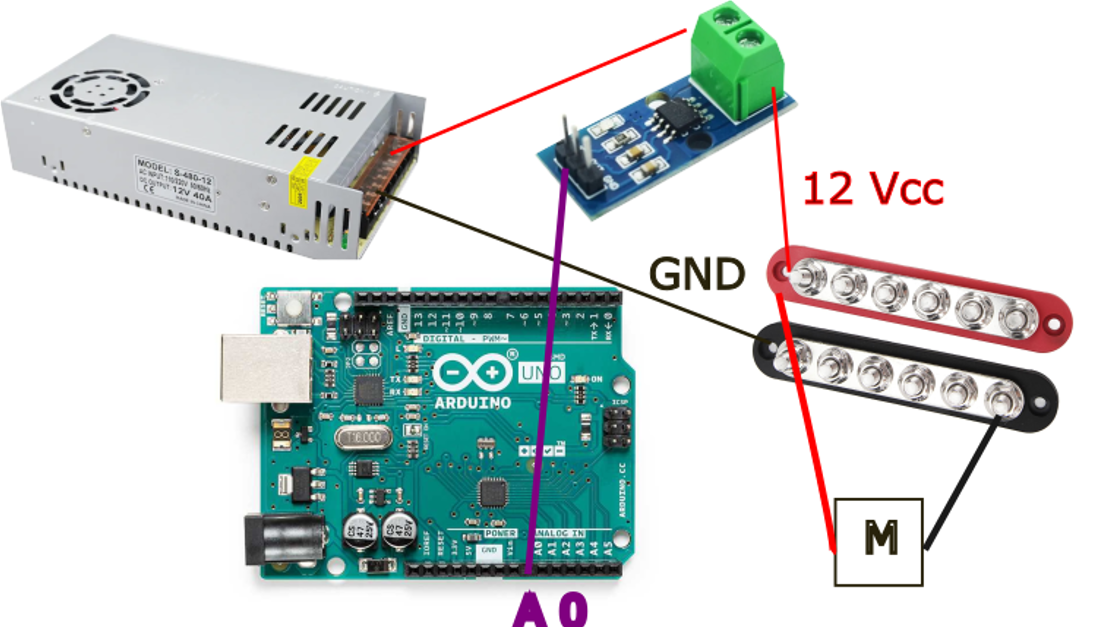
\includegraphics[width=0.7\linewidth]{images/SensorCorriente/screenshot016}
	\caption[Diagrama de conexión del sensor de corriente]{Diagrama de referencia de la arquitectura eléctrica. Se ilustra la trayectoria principal desde la fuente de poder hacia el sensor ACS712 y su posterior distribución al bus bar; los motores se representan en una configuración en paralelo. Cabe señalar que este esquema es simplificado y no muestra la totalidad de las conexiones de control.}
	\label{fig:screenshot016}
\end{figure}


Debido a que el sistema debe manejar corrientes considerables durante los picos de torque de todos los motores, la conexión física se realizó utilizando conductores de calibre \textbf{16 AWG}. Estos cables fueron fijados firmemente a las borneras del sensor. 

Es importante destacar que, para los alcances del presente periodo parcial, se validó exitosamente la etapa de transducción y comunicación entre el sensor ACS712, el microcontrolador Arduino Uno y la interfaz de usuario en LabVIEW. No obstante, como fase siguiente del desarrollo, se implementará una modificación en el hardware para automatizar el corte de energía. El sistema se programará para que, al detectar un umbral superior a los $14\,A$, se active una señal digital hacia un relevador encargado de interrumpir el suministro eléctrico hacia -y sólo- los motores, de tal manera, que la parte lógica pueda seguir funcionando para seguir brindando energía a la electrónica de control y reportar fallas a la interfaz de Labview o protocolo de comunicación que se esté utilizando. 

Está aún en decisión la tarjeta que será encargada de leer el sensor, pues se podría utilizar un Arduino Mega (que ya realiza las tareas del movimiento de los motores) o una ESP32 (que realiza cálculos con los encoders.) Dependiendo del nivel de tareas y uso de CPU total, se asignará la tarea al microcontrolador que esté menos saturado y pueda realizar la tarea con precisión.





\section{Interfaz de Monitoreo en Tiempo Real mediante LabVIEW}
% Habla sobre la visualización de datos y cómo la interfaz decide cortar la energía si se supera el límite de corriente.




\begin{figure}[h]
	\centering
	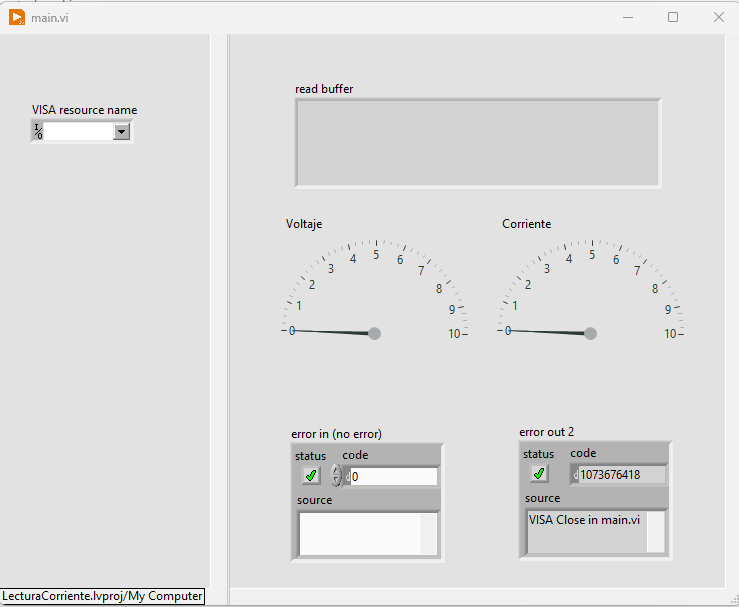
\includegraphics[width=0.7\linewidth]{images/SensorCorriente/screenshot018}
	\caption[Panel frontal de la interfaz para leer el sensor de corriente.]{Interfaz de usuario desarrollada en LabVIEW para la supervisión del sistema. Se observa el \textit{read buffer} para la depuración de datos seriales, indicadores tipo \textit{gauge} para la visualización en tiempo real del voltaje leído por el ADC y la conversión a corriente; además se muestra la gestión de recursos VISA para la comunicación con el Arduino Uno.}
	\label{fig:screenshot018}
\end{figure}

\begin{figure}[h]
	\centering
	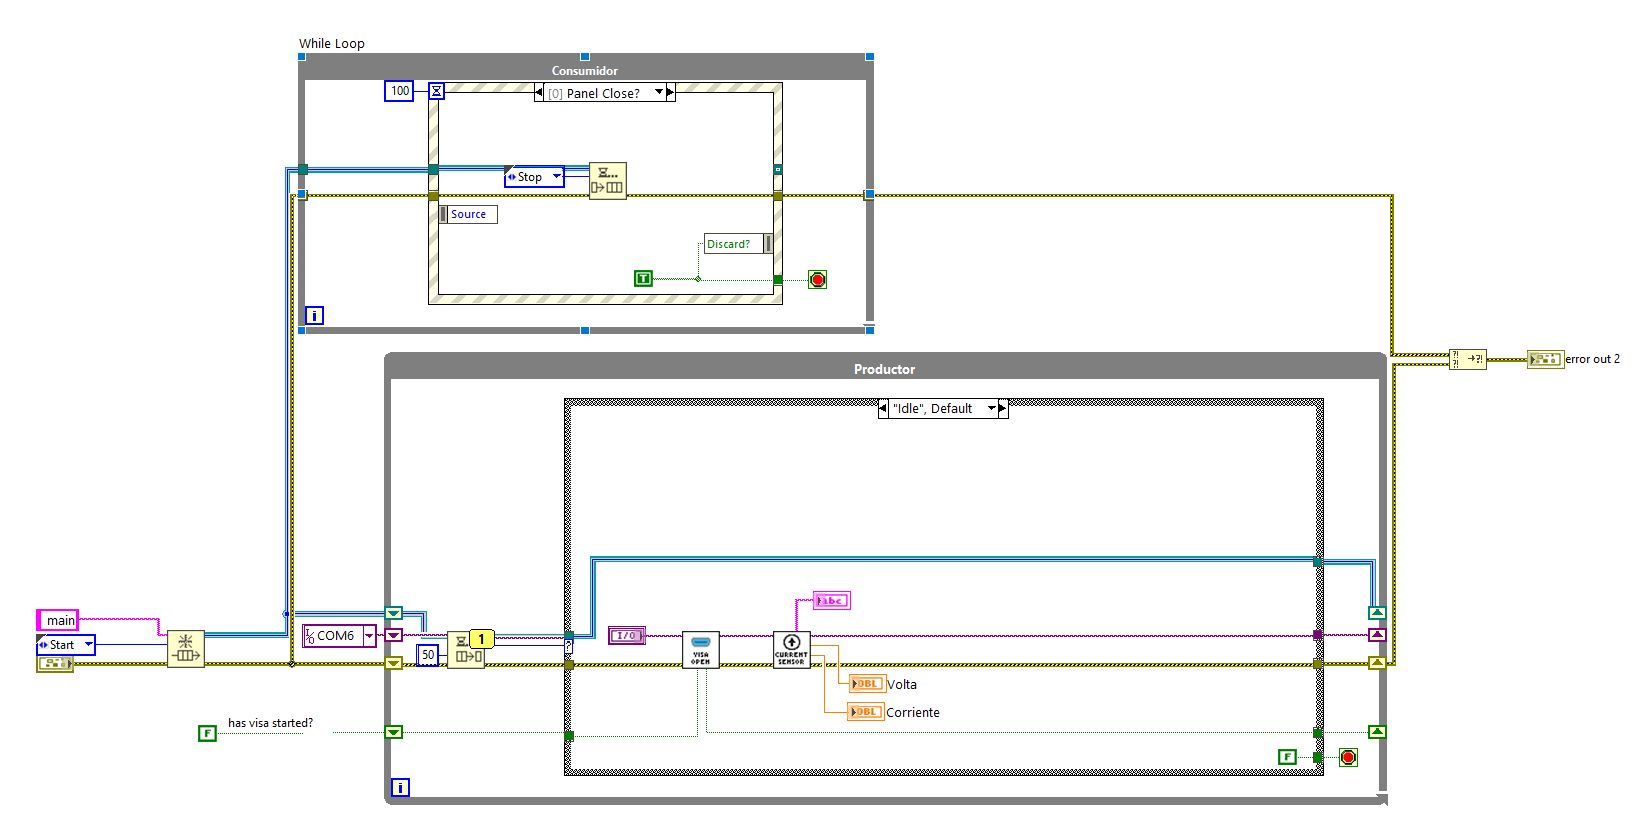
\includegraphics[width=1\linewidth]{images/SensorCorriente/screenshot019}
	\caption[Main del programa elaborado en Labview.]{Arquitectura del programa principal (\textit{Main VI}) basada en el patrón de diseño \textit{Queue Message Handler} (QMH). Se implementa una estructura de Productor/Consumidor donde el bucle consumidor gestiona la interacción del usuario con el panel frontal mediante una estructura por eventos, mientras que el bucle productor procesa las tareas de comunicación y cálculo a través de una estructura \textit{Case} alimentada por una cola de mensajes.}
	\label{fig:screenshot019}
\end{figure}

\begin{figure}[h]
	\centering
	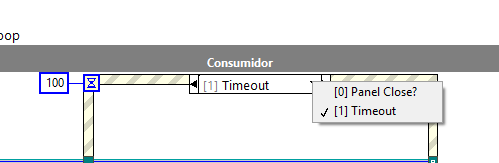
\includegraphics[width=1\linewidth]{images/SensorCorriente/screenshot021}
	\caption[Estructura del consumidor en Labview,]{La estructura del consumidor se encarga de los eventos que suceden dentro del panel frontal como lo son el timeout y el cierre del panel.}
	\label{fig:screenshot021}
\end{figure}



\begin{figure}[h]
	\centering
	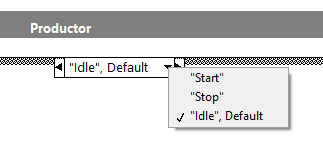
\includegraphics[width=1\linewidth]{images/SensorCorriente/screenshot020}
	\caption[Estructura del productor en Labview.]{Detalle de la estructura del Productor. Se observa el estado por defecto, configurado para ejecutarse cíclicamente cada 50\,ms. Esta configuración garantiza una tasa de refresco constante en los indicadores del panel frontal y permite una lectura fluida del puerto serie, manteniendo actualizados los gaugómetros.}
	\label{fig:screenshot020}
\end{figure}


\clearpage
\begin{resultadosFase}
	\begin{itemize}
		
		\item \textbf{Optimización del sistema de monitoreo:} La implementación de un único sensor ACS712 en la salida principal de $12\,V_{CC}$ de la fuente de poder resultó en una solución eficiente y centralizada, permitiendo supervisar el flujo total de energía hacia la etapa de potencia de los motores sin la complejidad de la lectura individual en los drivers.
		
		\item \textbf{Superioridad técnica del ACS712 sobre el BTS7960:} Se determinó que el sensor basado en efecto Hall ACS712 otorga una resolución y linealidad superiores en comparación con los pines del driver BTS7960. 
		
		\item \textbf{Prevención de daños térmicos y sobrecargas:} A partir del conocimiento de la corriente nominal de cada actuador, el sistema se configuró para identificar condiciones de riesgo. Esta capacidad de monitoreo asegura que los motores operen dentro de sus límites seguros, evitando el sobrecalentamiento o la destrucción de los devanados por efectos de corriente de rotor bloqueado.
		
		\item \textbf{Análisis dinámico mediante la HMI en LabVIEW:} La interfaz desarrollada permitió analizar de manera cuantitativa y visual cómo va a fluctuar la corriente ante la conexión de diferentes elementos de carga y durante los picos de arranque (\textit{inrush current}). 
		
		\item \textbf{Estabilidad de lectura mediante filtrado digital:} Gracias al algoritmo de promediado de 200 muestras integrado en el microcontrolador y visualizado en el \textit{read buffer} de LabVIEW, se logró una señal de corriente más limpia.
		
		\item \textbf{Implementación del circuito eléctrico:} Es necesario conectar un relé entre el sensor de corriente y la barra de bus que alimenta a los motores. Esta tarea se asignará al microcontrolador que esté menos saturado de tareas.
	\end{itemize}
\end{resultadosFase}